\chapter{Trajectory: a software process mining framework.} \label{trajectory}
As we saw in the Chapter \ref{related.work}, it is possible to infer and successively formalize software process by observing its artifacts, and particularly, recurrent behavioral patterns. The problem of finding such patterns is the cornerstone of my research. My approach to this problem rests on the application of data-mining techniques to symbolic time-point and time-interval series constructed directly from the real-valued telemetry streams provided by Hackystat.

\begin{figure}[tbp]
   \centering
   \includegraphics[height=65mm]{system_overview.eps}
   \caption{The high-level system overview. Software engineering process and product data are collected and aggregated by Hackystat and then used to generate temporal symbolic indexes. Data mining tools constrained by software engineering domain knowledge are then used for unsupervised patterns discovery. The GUI provides an interface to the discovered patterns and aids in investigation of a discovered phenomena.}
   \label{fig:system_overview}
\end{figure}


To investigate the requirements for a software tool that aids in the discovery of recurrent behavioral patterns in software process, I am designing and developing the ``Trajectory'' framework. A high-level overview of the framework is shown in Figure \ref{fig:system_overview} and resembles the flow of the ``Knowledge Discovery in Database'' process discussed by Han et al. in \cite{citeulike:709476}. As shown, the data collected by Hackystat is transformed into a symbolic format and then indexed for further use in data-mining. The tools, designed for data-mining, have a specific restrictions placed on the search space by domain and context knowledge in an attempt to limit the amount of reported patterns to useful ones. I am planning to design a GUI in a way that will allow easy access and modification of these restrictions. 

\section{Current state of development}
I started development of the Trajectory framework in early 2008 by designing a user interface for visual comparison of multi-variate time series. I called this package ``TrajectoryBrowser'' and called its results ``Software Trajectory Analysis''. The idea was to visualize software project metrics as a set of trajectories in 3D space, as opposed to the traditional 2D representation. The first \textit{TrajectoryBrowser} was an ad-hoc application based on the two technologies: Java3D for visualization and the UI, and the JADE multi-agent framework \cite{citeulike:1230319} for the data generation (see Figure \ref{fig:trajectory_progress} panels $a$ and $b$). While this first version fulfilled basic requirements for visualization, allowing trajectories to be visualized, it did not provide any means for quantifying similarities between trajectories or finding similar trajectories autonomously.

In order to introduce a metric and implement an indexing of temporal features, I then started experimenting with a naive application of Euclidean distance and later with spectral decomposition of time series through DFT. Unfortunately both methods were found to be inconsistent in their results and sometimes even misleading due to the noisy and bursty nature of temporal data generated by the software process. 

\begin{figure}[tbp]
   \centering
   \includegraphics[height=155mm]{trajectory_progress.eps}
   \caption{Screenshots of three versions of TrajectoryBrowser (panels $a$, $b$ and $d$) and the software process simulation (panel $b$). Simulated data was used for validation in early stages.}
   \label{fig:trajectory_progress}
\end{figure}

At the next iteration, inspired by its success in many applications and its robustness to noise, I implemented the Dynamic Time Warping (DTW) algorithm. This code was wrapped into the second, web-based version of TrajectoryBrowser (see Figure \ref{fig:trajectory_progress} panels $c$). The second version provided the user with the ability to visualize time-series intervals and quantify the similarity. Nevertheless, there was no implementation of the unsupervised similarity search provided.

In order to close this gap, I started developing an indexing module that uses sliding window and DTW. While working on this, I found another promising approach for the same task: PAA and SAX (see section \ref{paa} and \ref{sax}) approximations. The simplicity of these two methods allowed me to integrate them with my existed codebase almost instantly, delivering the third version of TrajectoryBrowser which I am currently using in my research. Sections \ref{indexing} and \ref{indexing_design} present the indexing mechanism and the index database design. 

\subsection{Temporal data indexing} \label{indexing}
The temporal data indexing starts with the data abstraction process shown at the Figure \ref{fig:data_flow}. Collected and aggregated by Hackystat, \textit{raw sensor data} and derived \textit{Hackystat Telemetry streams} are used as the data sources. Streams of individual events are retrieved from the Hackystat Sensorbase, then sorted by activity types, tokenized, and finally converted into symbolic time point (\textit{Events}) and time-interval (\textit{Episodes}) series by following a user-defined taxonomy mapping. By performing a user-configured PAA and successive SAX approximations, Hackystat Telemetry streams are converted into a temporal symbolic format. This symbolic data, in turn, are getting indexed and stored in the dedicated relational database for future use in data mining.

\begin{figure}[tbp]
   \centering
   \includegraphics[height=85mm]{data_flow.eps}
   \caption{Overview of the data abstraction from the the low-level process and product artifacts collected by Hackystat (left side) to the high-level symbolic time-point and time-interval series stored in the Trajectory data repository.}
   \label{fig:data_flow}
\end{figure}

I have not experimented with symbolic abstraction and mining of the raw sensor data yet, but this approach has a solid foundation provided by Hongbing Kou, in his thesis \cite{citeulike:2703162}. In his work, he was able to infer TDD behaviors by using a technique called Software Development Stream Analysis (SDSA) which is very similar to mine. Within SDSA, low-level software process data was first converted into symbolic Episodes first. Next, sequences of Episodes (candidate patterns) were matched (aligned) to the set of the known TDD temporal rules (patterns), and if they were found to satisfy TDD rules (having sufficient support), the generative process was inferred as TDD.

\begin{figure}[tbp]
   \centering
   \includegraphics[height=60mm]{indexer.eps}
   \caption{Overview of the current implementation of Hackystat Trajectory framework.}
   \label{fig:indexer}
\end{figure}

The indexing of Telemetry streams I have implemented with a sliding window, PAA, and SAX. I am using a sliding window approach following \cite{citeulike:2821475} for generating a set of subsequences from a real-valued stream. Each of the subsequences is then normalized and converted into a symbolic representation with PAA and SAX. This symbolic representation and the position information is then stored in the relational database. For index manipulation and data retrieval I am leveraging SQL. Figure \ref{fig:indexer} presents the current software system overview.

\subsection{Index database design} \label{indexing_design}
Figure \ref{fig:trajectory_db} presents the TrajectoryDB database schema in detail. This schema was designed with two main requirements in mind. First, it must be able to hold a local copy of Telemetry streams due to the high time cost of querying Telemetry service remotely. Second, it must support implemented KDD algorithms through optimized SQL queries. Both goals were archived, resulting in the extremely high turn-around speed for both indexing and querying.

\begin{figure}[tbp]
   \centering
   \includegraphics[height=200mm]{trajectory_db.eps}
   \caption{The database schema used for the Hackystat Telemetry data retrieval and indexing in the pilot project.}
   \label{fig:trajectory_db}
\end{figure}

The current version of Hackystat is based on a Service-Oriented architecture, and in order to retrieve a Telemetry data one must query Telemetry service over network. My initial implementation of indexing required network queries for the each of the indexing passes and was significantly affected by the network lag to my remote location and the amount of data needed to be retrieved for each pass. To overcome this issue I have a software module which provides ``caching'' and which incrementally updates Telemetry streams data locally. The \textit{Project, User, Member, Chart, Chartvalue} and \textit{Download} tables (located at the upper part of the Figure \ref{fig:trajectory_db}) are designed to store the Telemetry data locally. The system performs incremental update of the streams over time by reading the \textit{Download} table, which keeps track of updates.

The telemetry streams indexing is performed on demand. For each of the indexes a sliding window size, PAA size, and an alphabet must be specified. Following Lin \& Keogh \cite{citeulike:2821475}, in order to investigate the sensitivity and selectivity of different approximation levels, I have conducted a number of experiments with various alphabets. Individual alphabets for each of the data streams (\textit{Build, Coverage} etc.) and \textit{Universal Telemetry Alphabet} (see example for five letters alphabet at the Figure \ref{fig:distribution}, panel $a$) were built and tested for indexing. These custom alphabets, and the original SAX alphabet, based on the Normal distribution, are kept in the \textit{Sax\_alphabet} and \textit{Alphabet\_cut} tables. 

The \textit{Sax\_top\_index} table is a ``binder'' which keeps information about all indexes ever built. The \textit{Sax\_index\_chart} table keeps track of all indexes built for a particular chart and a timeframe. \textit{Sax\_motif} and \textit{Sax\_motif\_entry} tables separate heavyweight symbolic motifs and lightweight offset ``information'' reducing the database size and optimizing data analysis and retrieval. 

This database schema was found optimal for easy retrieval of any kind of information needed for streams comparisons or clustering. By running a single query it is possible to retrieve a vector of most frequent motifs for each of the streams or find a set of motifs shared between streams.

\section{TrajectoryBrowser}
As mentioned before, the current version of TrajectoryBrowser was created in order to visualize telemetry streams along with temporal features found through indexing. It provides easy navigation within indexes and is capable of displaying multiple telemetry streams with highlighted features. By viewing the same motif entry across multiple streams it is possible to guess information about coincidence of entries, as an example, see Section \ref{pilot.evaluation}, for sequential ``growth'' pattern finding experiment.

\begin{figure}[tbp]
   \centering
   \includegraphics[height=185mm]{distribution.eps}
   \caption{The distribution of the Hackystat Telemetry data. While individual telemetry streams (panel $b$, left three plots for each stream represent raw data, right three plots - Z-normalized data) show different data distributions, the combined and normalized data (panel $a$) close to the normal distribution. Combined data was used for creation of the \textit{Universal Telemetry SAX alphabet}.}
   \label{fig:distribution}
\end{figure}

\section{Future development roadmap}
As I pointed before, the current version of the TrajectoryBrowser and analyses do not support processing of low-level raw Hackystat data and analyses based upon them. I have already started the development of such module along with extending a database schema for storing raw data, its approximation, and taxonomy. Once these components are in place, I will start developing data mining algorithms for Events and Episodes using the discussed temporal data mining algorithms. Once all major software pieces are in place, I will focus on the experimental evaluation of the system and improving the usability of the GUI.